% %!TEX root = ../../../main.tex
% \section[Coupling \Nds to Optical Antennas]{Coupling \Nds to Double Bowtie Antenna Structures} \label{sec::coupling_antennas}
%
% 	Plasmonic nanoantennas are very recent devices designed to efficently convert freely propagating optical radiation into localized energy and vice versa \cite{Optical Antennas, Palash Bharadwaj, Bradley Deutsch, and Lukas Novotny, nancy::77, nancy::78}. Leveraging this unique property, integrating \sivs with optical antennas creates coupled systems with a range of desireable features. These include enhanced \pl emission and the ability to tailor \pl spectra of the integrated emitters. The latter can be achieved by tuning the physical design parameters of the system including antenna geometry and emitter placement.
%
% 	In this chapter we report on our efforts aimed at enhancing the properties of \sivs by coupling them to optical double bowtie antennas. To this end we transfer selected \nds containing \sivs to the target antenna structure using \pp methods. After successful coupling we investigate the integrated structure experimentally. In addition to that we successfully relate some of our results to theoretical predictions.
%
% 	In the following we give a short discussion of the most important properties of optical antennas. Then we sketch the actual coupling process and report on the optical properties of the resulting integrated structure.
%
% 	\subsection{Plasmonic Antennas}
%
% 		Optical nanoantennas act as convertes between propagating and localized electro-magnetic fields. Thus, they can be used efficiently to couple photons in and out of nanoscale objects \cite{Curto2010}. Due to their small physical sizes, comarale or smaller than the \wl of visible light, they are capable of focusing optical fields to subdiffraction-limited volumes, offering the ability to manipulate electromagnetic fields at nanoscales \cite{Curto2010::3, nancy::78}. This property, dubbed sub-wavelength confinement, has successfully been exploited to enahnce the excitation and emission of quantum emitters \cite{Curto2010::4, Curto2010::5, Curto2010::6, Curto2010::7} and to modify their spectra \cite{Curto2010::8}. Resulting practical applications include near-field optical microscopy \cite{nancy::79}, surface enhanced spectroscopy \cite{nancy::80, nancy::81} and molecular sensing \cite{nancy::82}.
%
% 		A nanoantenna is a nanostructure made from materials such as noble metals like gold or silver. These metals have in common that they are very susceptible to being polarized by electro-magnetic fields. When illuminated by the incident electromagnetic radiation causes electrons in the metal to behave as a plasma that tends to move with respect to the atomic lattice. As a result excess charge at the opposite surfaces of the material accumulates and the material becomes temporarily polarized until restoring forces equillibrate the charge distribution.
%
% 		Thus incident light of a given frequency induces oscillations in the free electron gas density in the surface layers of the metal. At resonance these light-induced oscillations exhibit modes of standing waves. The quasi-particles associated with these modes are known as \lsps (\LSPs).
% 		For an in-depth treatment of \LSPs in the context of nanoantennas we refer the reader to \cite{nancy::thesis} and references therein.
%
% 		Here it suffices to say, that \LSPs facilitate the deciding property of optical antennas: Converting electromagnetic energy from the far-field into localized energy in the near-field. This allows, in combination with the high collection-efficencies of nanoantennas, to efficiently couple visible radiation with wavelenghts of hundres of nanometers, into small effective spatial volumes of only a few nanometer in diameter.
%
% 		To create a controlled hot-spot several antenna designs are possible. In the context of this thesis we rely on double bowtie antennas available via a collaboration with \nancy. \autoref{fig::double_bowtie_antenna_schematic} illustrates the typical bowtie antenna.
%
% 		\begin{figure}[thp]
% 				\centering
% 				\testbox{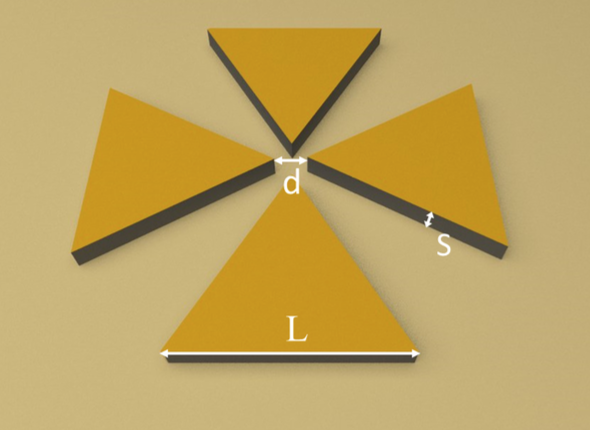
\includegraphics[trim = 0 0 0 0,  clip= true, width = 0.5\textwidth]{./pics/double_bowtie_antenna_schematic.png}}
% 				\caption[Schematic of a double bowtie antenna]{Schematic of a double bowtie antenna \cite{nancy::thesis, Rahbany2015, Rahbany2016}.}
% 				\label{fig::double_bowtie_antenna_schematic}
% 		\end{figure}
%
% 		This antenna design utilizing a symmetric arrangement of four identical triangle-shaped blocks, separated by a small gap. This setup allows \LSP modes local to individual blocks to couple with each other resulting in the formation of an intense hot-spot in the center area \cite{nancy::85}, see \autoref{fig:double_bow_tie_hotspot}. The actual electromagnetic response of a double bowtie nanoantenna depends on its physical design parameters such as gap size, material used, geometry and size. Furthermore, properties of incident light such as \wl and polarization determine antenna operation.
%
% 		\begin{figure}[thp]
% 				\centering
% 				\testbox{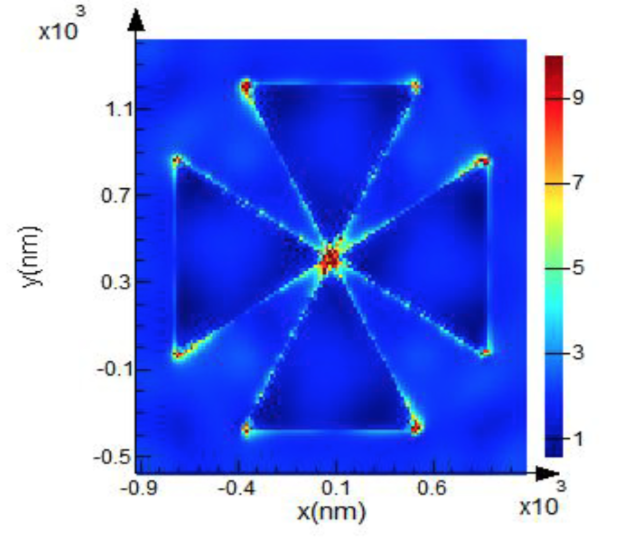
\includegraphics[trim = 0 0 0 0,  clip= true, width = 0.5\textwidth]{./pics/antenna_fdtd_simulation_field.png}}
% 				\label{fig::double_bow_tie_hotspot}
% 				\caption[Hot-spot of a double bowtie antenna]{Simulation result of the electric field map of a gold double bowtie nanoantenna \cite{nancy::thesis, Rahbany2015, Rahbany2016}. The structure has gap of $d = \SI{150}{nm}$, a side length of $L = \SI{2}{\micro\meter}$ and a thickness of $S = \SI{60}{nm}$. The center of the antenna exibits an area of pronouced focus, the so-called hot-spot.}
% 		\end{figure}
%
%
% 		The improved electromagnetic field at the center of a metallic nanoantenna can be used to increase the spontaneous emission rate of emitters emitting at frequencies close to the resonance frequency of the antenna. This result is the known as Purcell effect \cite{nancy::86}. The gap between the antenna arms acts as a resonant cavity providing a strong near field interaction with the emitter. This interaction modiefies the density of states of the system, effectively providing additional modes for the emitter to decay into, thus amplifying its total decay rate. The amplification affects both radiative and non-radiative decay.
% 		The magnitude of the amplification for an emitter is quantified by the ratio of its enhanced decay rate to its free space decay rate, known as the Purcell factor $F_p$. This factor is proportional to $Q/V_{eff}$ where $Q$ denotes the quality of the antenna and $V_{eff}$ the volume of the hot-spot. Thus antenna desing must optimize $F_p$ as a necessary condition for significant enhancement of \fl emission.
%
% 		In addition to the antennas local field enhancment, the emitters original quantum yield $\eta_0$ influences the overall effectiveness of the emission enhancement. From theoretical considerations \cite{nancy::thesis, nancy::140, nancy::162, nancy::163}, the modified quantum efficiency $\eta$ of the combined system consisting of emitter and antenna can be obtained as
%
% 		\begin{equation}
% 			\eta = \frac{\eta_0}{\frac{1-\eta_0}{F_p} + \frac{\eta_0}{\eta_{ant}} },
% 		\end{equation}
%
% 		where $\eta_{ant}$ denotes the fraction of \fl which is not dissipated through losses in the metal of the antenna. It is clear that an emitter with $\eta_0 \to 1$ will not profit from the Purcell effect. On the contrary, for realisitc antennas with $\eta_{ant} < 1$ antenna-induced losses reduce the overall quantum yield $\eta$. Consequently poor emitters with low initial $\eta_{0}$ stand to profit the most from antenna-emitter coupling provided antennas are engineered well, \i.e.\ they maximize their Purcell Factors and minimize their losses. For an in-dept review
%
% 		The presented considerations illustrate that due to their relatively low quantum efficiency, \sivs are excellent candidates for coupling with antennas. Thus it is promising to expliot the improved electromagnetic field at the center of a double bowtie antenna to enhance the spontaneous emission rate of \sivs and thus improve their merit as \spss.
%
% 	\subsection{Plasmonic Antenna Design and Simulation} \label{sec::structure_antenna}
%
% 		 To couple \sivs to optical antennas, we work with gold double bowtie antennas on a gold substrate. In comparison with triangular, or single bowtie antennas, double bowtie antennas offer significantly improved intensity enhancements. Antennas were provided by \nancy in a joined effort to explore the possibilities of combining antennas with \sivs. The antennas themselves were fabricated using electron beam lithography, a technique suitable to imprint predetirmined patterns onto a suitable substrate with nanoscale resolution \cite{nancy::232}. \autoref{subfig::antenna_structures_sem} shows a SEM image of an array of antenna structures of various sizes. In \autoref{subfig::antenna_one_structure_sem} a detail of an individual double bowtie antenna is shown. It can be seen that the double bowtie antenna is placed in the center of another structure, a so-called bulls-eye antenna, consisting of multiple concentric gratings. When illuintated by a laser at a proper angle, the gratings excite surface plasmon polaritons (SPPs) which are directed towards the center of the structure. If a double bowtie antenna is present in the center, SPPs can interact with the \LSPs of the double bow tie, leading to an even stronger localization of electromagnetic fields in the gap of the bowtie. While this interaction certainly merits exploration in the context of enhancing \sivs, we omit the excitation of SSPs in our first exploration of the couling of \sivs and antennas. Thus the presence of the gratings can be ignored for our purposes. The reader interested in the details of bulls-eye antennas and their properties is referred to \cite{nancy::thesis}.
%
% 		 		\begin{figure}[htp]
% 		 			\begin{subfigure}[t]{ 0.49\linewidth}
% 		 				\centering
% 		 				\testbox{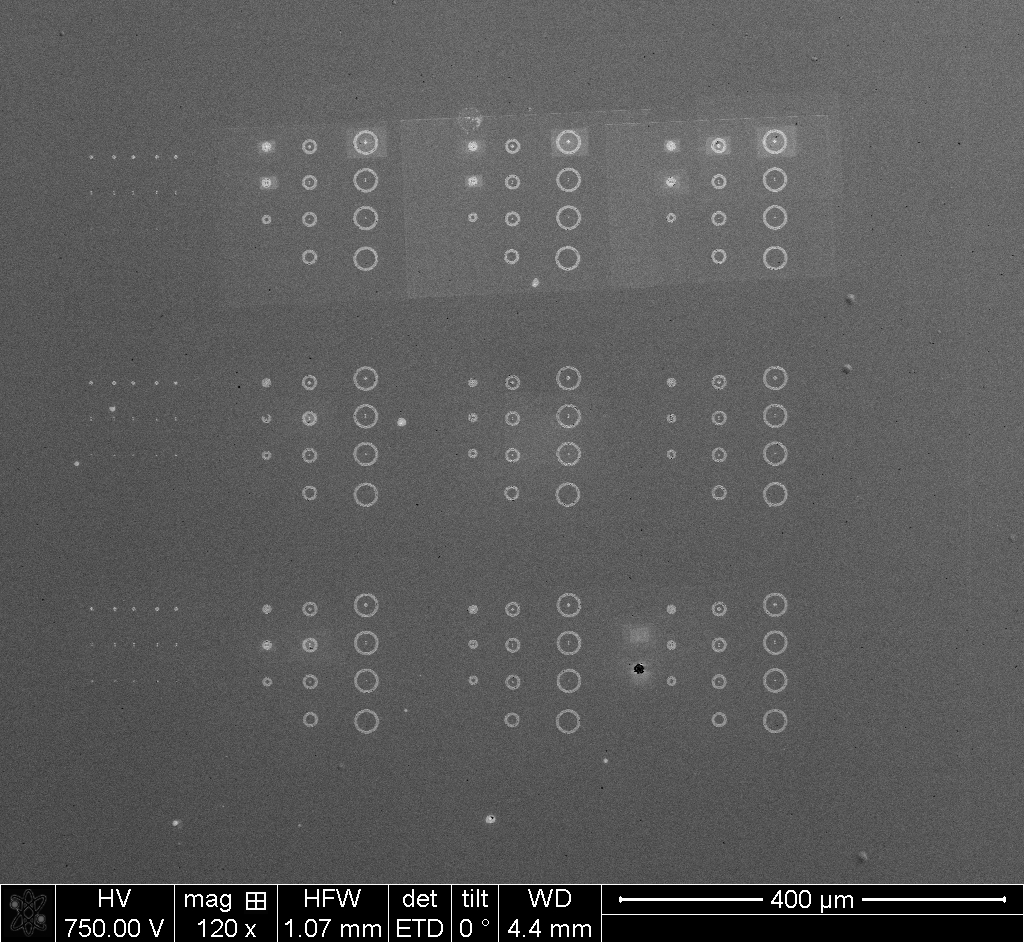
\includegraphics[trim = 0 0 0 0,  clip= true, width = 0.7\textwidth]{./pics/Antenna2_upper_right_150923_01.png}}
% 		 				\caption{}
% 		 				\label{subfig::antenna_structures_sem}
% 		 			\end{subfigure}
% 		 			\hfill
% 		 			\begin{subfigure}[t]{ 0.49\linewidth}
% 		 				\centering
% 		 				\testbox{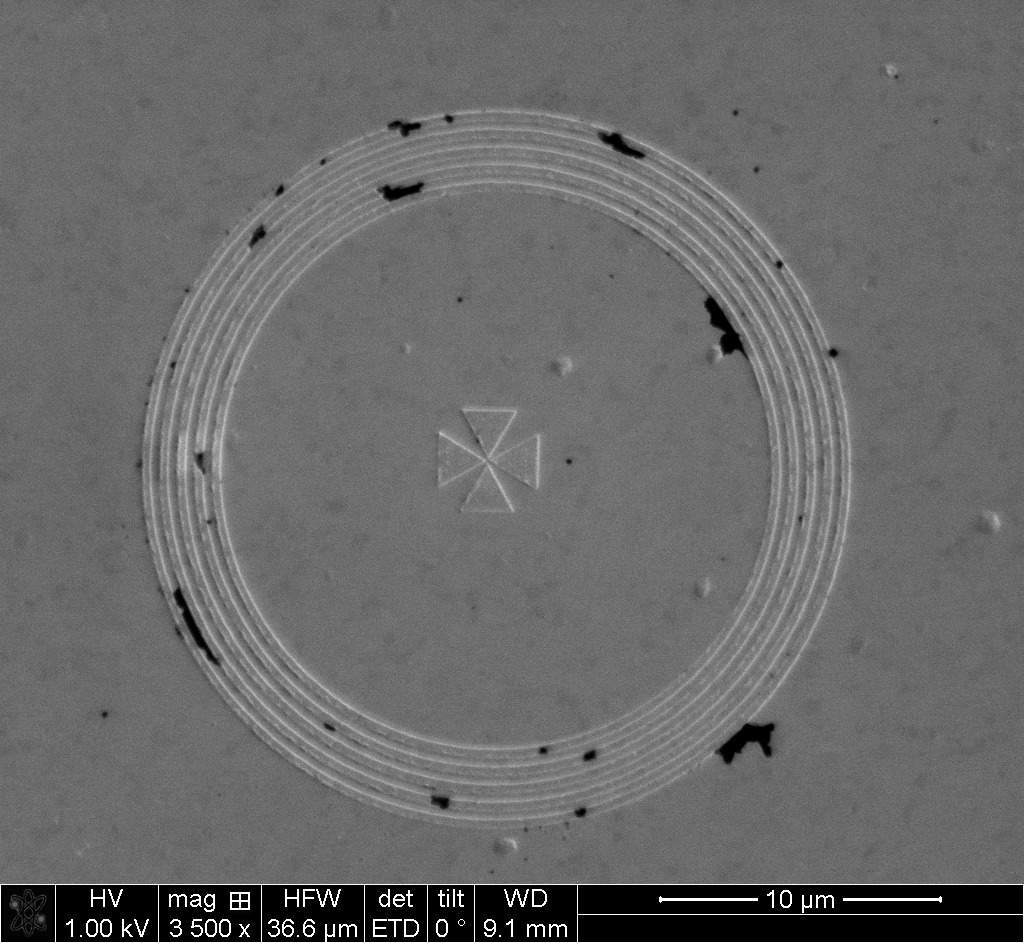
\includegraphics[trim = 0 0 0 0,  clip= true, width = 0.7\textwidth]{./pics/Ir27M_mitte_213_151111_13.jpg}}
% 		 				\caption{}
% 		 				\label{subfig::antenna_one_structure_sem}
% 		 			\end{subfigure}
% 		 			\caption[SEM images of double bowtie structures.]{SEM images of antenna structures. (a) Overview of a field of antenna structures exhibiting various dimensions. (b) Detail of one antenna sturcture. In the middle the double bowtie design is visible. A grating structure consisting of multiple gratings is surrounding it.}
% 		 		\end{figure}
%
% 		To effectively enhance the emission of an emitter by coupling it to an optical antenna, the emission \wl must match the resonant \wl of the antenna. In the context of \sivs a value of \SI{738}{nm} is required. Since this value can be considered constant, the design parameters of the antenna must be choose such, that the resulting resonance matches it. An additional constraint is placed on the size of the antenna gap, since it must be big enough to accomodate \nds hosting \sivs, the former are around \SI{100}{\nm} in size. However, it cannot be choosen arbitrarily big, since bigger gaps lead to larger effectiv volumes and thus smaller Purcell Factors.
%
% 		Using finite time difference domain (FDTD) simulaton deploying Lumerical Software the design space of gold double bowtie nanoantennas on a gold substrate was explored \cite{nancy::thesis}. Although we initially attempted to simulate antennas without a \nd present in the gap, it was subsequently discovered that its ab initio inclusion yielded superior results. Thus to determine usable design parameters for our purposes, an integrated system combining antenna and \nd was used. To better mimick experimental conditions and associated imprefections, the \nd was placed slightly off-center in the gap.
%
% 		In a series of simulation it was established that a gapsize of $d = \SI{150}{nm}$, a side length of $L = \SI{2}{\micro\meter}$ and a structure thickness of $S = \SI{60}{nm}$ are feasible parameters as refered to in \autoref{double_bowtie_antenna_schematic}. The simulation required the index of refraction for gold which was taken from Palik \cite{Palik, E. D. Handbook of optical constants of solids. 3, (Academic press, 1998)}.
%
% 		The resulting geometry hosting a \nd is capable of producing a suitable hotspot when excited.
%
% 		\begin{figure}[htp]
% 				\centering
% 				\testbox{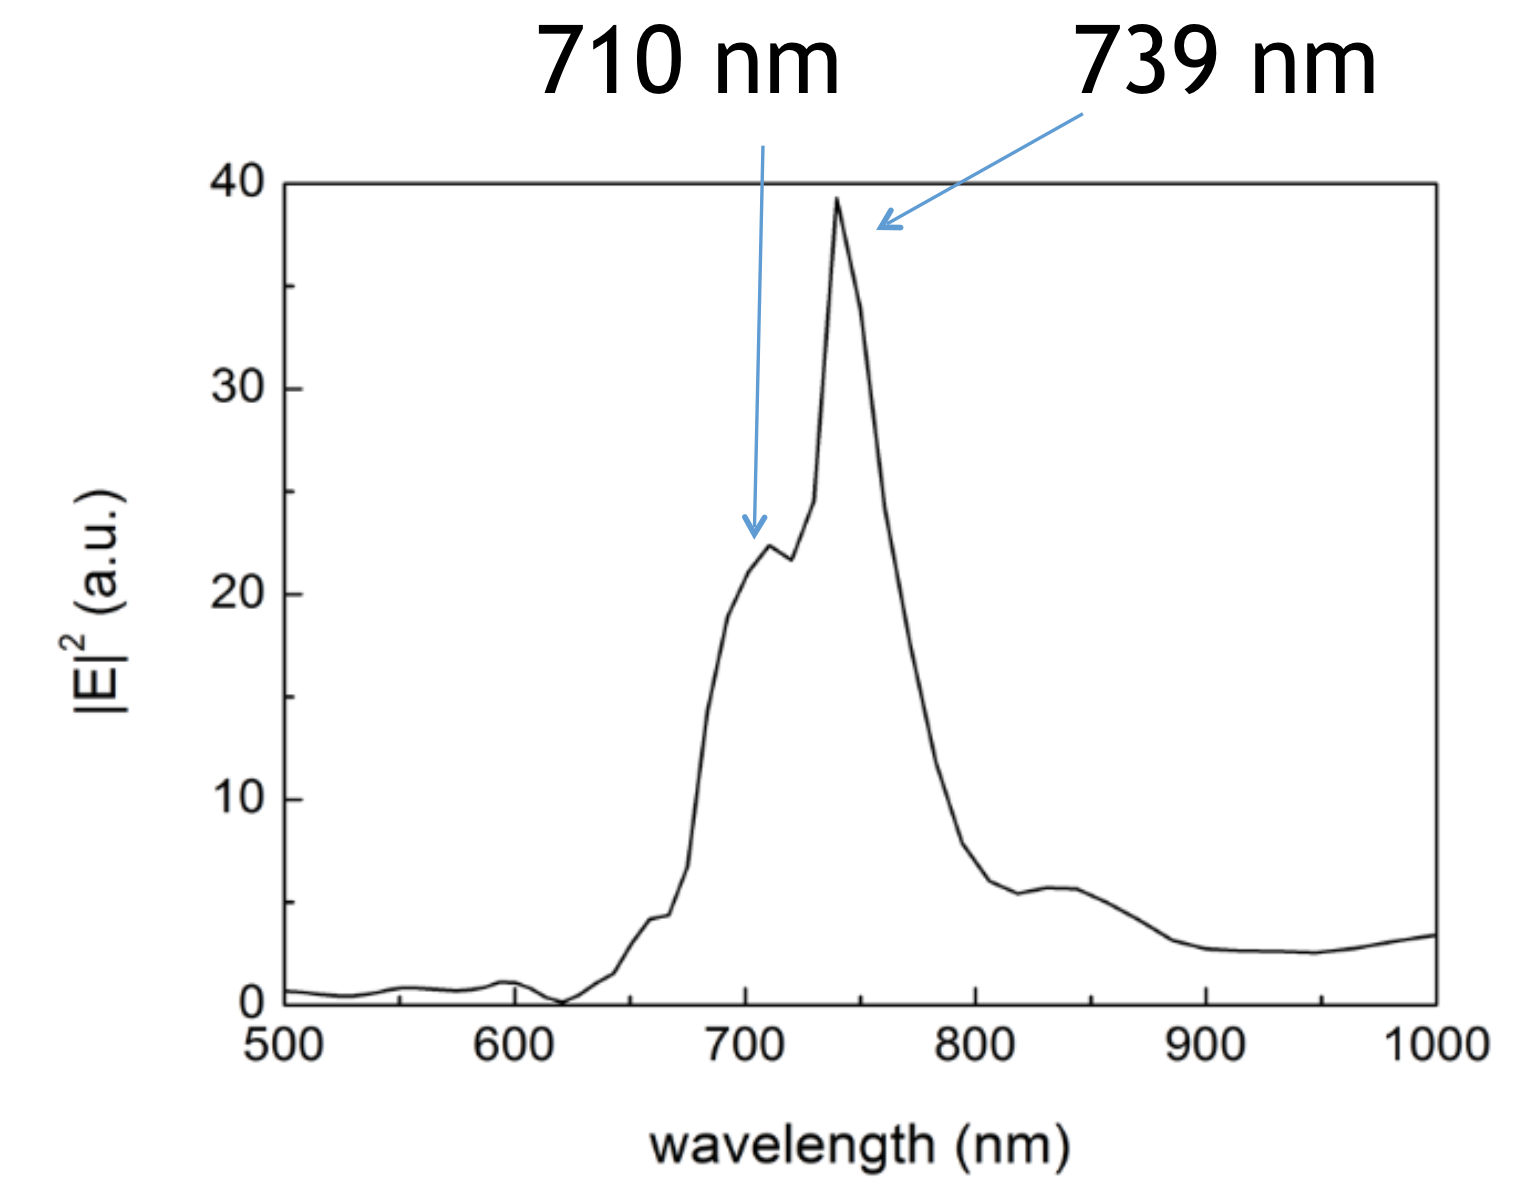
\includegraphics[trim = 0 0 0 0,  clip= true, width = 0.5\textwidth]{./pics/antenna_fdtd_simulation_spectrum.png}}
% 			\caption[Simulation of the resonance spectrum of a double bowtie antenna]{FDTD simulation of the electric field intensity of a double bowtie nanoantenna as as a function of the \wl of incident light. Two peaks are identified. The major peak corresponds exceptionally well with \siv emission at \SI{738}{nm}. The minor peak is attributed to the presence of a \nd.}
% 			\label{fig::antenna_fdtd_spectrum}
% 		\end{figure}
%
% 		Finally, to pin-point the resonant \wl for the antenna hosting a \nd, the electric field intensity is simulated as a function of the \wl of the incident light. The resulting spectrum is shown in \autoref{fig::antenna_fdtd_spectrum}. Two resonant peaks are found. The intense major peak at \SI{739}{nm} coincides exceptionally well with the \siv emission wavelength \SI{738}{nm} indicating successful antenna design. In addition to the major peak, an additional minor mode at a lower wavelength of \SI{710}{nm} is found \cite{Rahbany2016}. We remark that if the \nd in the gap of the antenna is removed from the simulations, the minor feature vanishes. Thus the additional peak is well-attributed to the presence of the \nd.
%
% 		In summary, the combined simulation results suggest, that the engineered system of nanoantenna and \nd is well suited to effectively enhance the emission from an \siv hosted in the \nd. In the following sections we report on the experimental realization of this preposition.
%

	\subsection{\siv in a Plasmonic Double Bowtie Antenna}

		In the following we report on our attempts to couple \sivs to gold double bowtie nanoantennas in order to study the properties of the resulting integrated system. Ideally, a suitable \nd containing exactly one \siv is placed in the center of the antenna. The term suitable is used to summarize both desirable spectroscopic properties such as narrow-bandwith saturated single-photon emission as well as technical requirements such as \nd size and degree of isolation on the surface. Naturally, the odds of identifying and adressing a \nd fullfilling all these criteria simulatneously are small. As a result identifying a perfect canditate for coupling is prohibitively time-consuming.

		To mitigate this difficulty we decided to relax the condition of exactly one \siv per \nd and initiate our explorative work with \nds containing several, potentially many active \sivs. Relying on \gtz measurments we identify two interesting classes of \nds. The first class consists of \nds containing large ensembles of \sivs acting as coherent emitters. The \fl light recieved from large ensemble of emitters is mainly coherent, leading to a flat response in the \gtz function. The second class of \nds we investigate features \nds hosting multiple \sivs. As a result relevant \gtz measurments report weak but discernable anti-bunching dips. Both classes have incommon that relevant \nd specimen are significantly easier to obtain than \nds containing singleton \sivs. Thus \nds containing ensembles of \sivs as well as \nds containing few \sivs are both valid starting points for our work. It is likely that the experience gained during our preliminary explorations will be valuable once \nds containing singleton \sivs become available.

		In the following sections we report on our efforts to couple \nds containing \sivs to antennas. We illustrate the coupling process and its challenges and discuss relevant results regarding the coupling of \nds of the classes described above. We close the chapter with a short discussion and suggestions for further research \todo{irgendwo uebersichts lsm scan reintun}.

		% 
		%
		% % Einleitung
		% In the following we give specific details on the challenging process of coupling \sivs to plasmonic double bowtie antennas. Furthermore, we report our results regarding spectroscopic measurements of coupled emitters.
		% \\
		% % additional methods
		% We performed coupling the nanodiamonds containing \sivs in two approaches:
		% First we chose a \nd containing several \sivs for \pp and afterwards a \nd containing a single \siv.
		% As mentioned before, single \sivs may be damaged by the electron radiation in the SEM during \pp and stop emittig \pl light.
		% Hence, we decided to run first experiments with \nds containing multiple \sivs.
		% This approach has the advantages that we are able to gain experience in the execution of the \pp process without the risk of permanently damaging the emitter and therefore rendering the tedious \pp process futile.
		% For measurements of the intensity enhancement by the antenna, a single emitter is necessary.
		% However, the antenna's influence on the \siv spectrum can be studied when serveral emitters are present.
		% Therefore, studies of the spectrum are performed in this first approach.
		% \\
		% After we gained experience with the first approach, we  searched for a suited \nd containing a single \siv.
		% The aim was to perform saturation and second order correlation measurements to probe single SiV centers, and consequently quantify the exact Purcell enhancement imposed by the nanoantenna on a single photon emitter.
		% % However, the challenges for experiments with a single \siv are magnitudes bigger than for multiple \sivs.


		\subsubsection{\Nds Containing Ensembles of \sivs Coupled to Antennas}\label{subsubsection::antenna_multiple_sivs}

			The \nds exploited for the approach of coupling multiple \sivs to an antenna were produced by a wet-milling process from a CVD diamond film\footnote{wet-milling performed by \muzha, diamond film grown by group of \williams} .
			The solution of \nds which exhibit a median size of \SI{100}{nm} were spin-coated on an iridium substrate treated with Piranha etch.
			To ensure that a pre-characterized nanodiamond exhibiting preferred optical properties (eg. narrow linewidth, high count rate) is later found again, the iridium substrate was engraved with reference cross markers produced by a focused ion beam prior to the spin-coating process.
			After spin-coating, the sample was placed in an oven for 3 hours at \SI{450}{\celsius} to oxidize the surface and remove any residual graphite and amorphous carbon.

			% position
			To determine the position of \nds on the original substrate, first a scan with a commercial \lsm (LSM) was performed as described in \autoref{subsec::position}.
			\autoref{subfig::cross_laser_scan} shows a part of an obtained LSM image.
			The cross marker can easily be identified, the black dots are \nds.
			After transferring the sample into the confocal setup, confocal \fl scans of the corresponding areas are performed to identify \nds containing active emitters.
			The scanned area is shown in \autoref{subfig::pp_pl_scan}. It corresponds to the area shaded blue in \autoref{subfig::cross_laser_scan}. Thus, upon close inspection some of the bright spots appearing in the \fl scan can be associated with selected \nds in \autoref{subfig::cross_laser_scan} by eye. The correspondence between the SEM and LSM images in conjunction with the cross-markers on the substrates allows to precisely locate preselected \nds containing suitable emitter in the SEM.

			\begin{figure}[htp]
				\begin{subfigure}[t]{ 0.49\linewidth}
					\centering
					\testbox{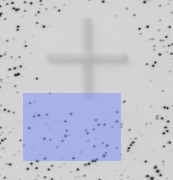
\includegraphics[trim = 0 0 0 0,  clip= true, height = 0.5\textwidth]{./pics/M05-13_structure3_stitch_crop_area.jpg}}
					\caption{}
					\label{subfig::cross_laser_scan}
				\end{subfigure}
				\hfill
				\begin{subfigure}[t]{ 0.49\linewidth}
					\centering
					\testbox{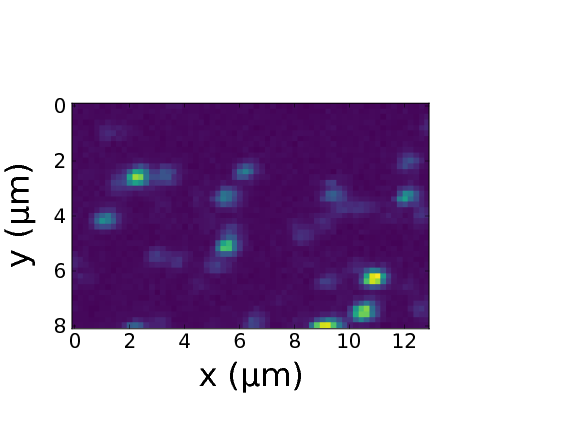
\includegraphics[trim = 0 20 70 50,  clip= true, height = 0.5\textwidth]{./pics/scan_xy-32_2APD_mum_noscale.png}}
					\caption{}
					\label{subfig::pp_pl_scan}
				\end{subfigure}
				\caption[Localizing suitable \nds]{(a) Picture recorded with a commercial high resolution laser scanning microscope. Black dots are individual \nds. The cross-marker serves as an orientation aid. The area shaded in blue represents the \pl scan in image (b). (b) \Pl scan of a
				$\SI{8}{\micro\metre} \times \SI{13}{\micro\metre}$. }
			\end{figure}

			% preselection
			% Fig. 1c shows an example of a PL scan where bright spots (highlighted by the red circles) correspond to nanodiamonds with PL in the SiV center spectral range. To further verify the presence of SiV centers, PL spectra at room temperature are recorded.
			\autoref{fig::spectrum_nd_multiple} shows the spectrum stemming from one such preselected \nd.
			The ZPL peak exhibits a \wl of \SI[separate-uncertainty = true]{738.55\pm0.01}{nm} and a \lw of \SI[separate-uncertainty = true]{5.0\pm0.03}{nm}.
			These numbers correspond well to the ZPL of unstrained SiV centers and therefore allows us to deduce that the studied nanodiamond contains at least one SiV center. Photon autocorrelation measurements revealed that the \nd contains multiple \sivs.

				\begin{figure}[htp]
						\centering
						\testbox{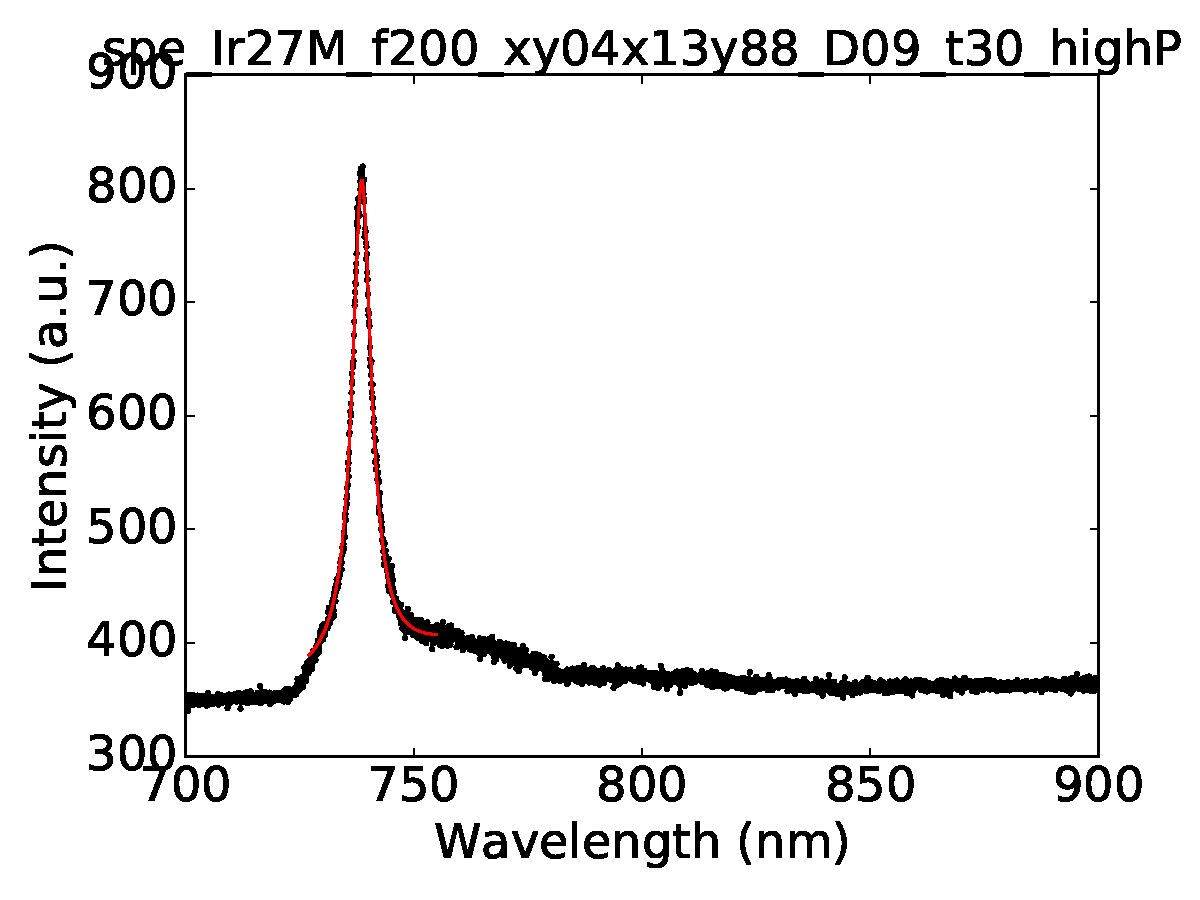
\includegraphics[trim = 0 0 0 0,  clip= true, width = 0.7\textwidth]{./pics/spe_Ir27M_f200_xy04x13y88_D09_t30_highP_fit.pdf}}
						\label{fig::spectrum_nd_multiple}
					\caption[Spectrum of a \nd containing at least one \siv]{PL spectrum of the emitter in the preselected nanodiamond at room temperature. Black: experimental results; red: fit to experimental data, which yields a \ZPL \cwl of \SI[separate-uncertainty = true]{738.55\pm0.01}{nm} and a \lw of \SI[separate-uncertainty = true]{5.0\pm0.03}{nm}. The narrow \cwl and the almost invisible sideband makes this \nd an excellent candidate for coupling to an antenna.}
				\end{figure}

			% A long pass filter (λ = 720 nm) is placed in the detection path to suppress any signal stemming  from the laser.. During the PL scan, the laser spot scans the surface and the emitted PL is recorded by the APD. In front of the APD a 730-750nm bandpass filter is installed. The center wavelength of the zero-phonon line of an SiV center is located at around 738 nm. Therefore, if a nanodiamond contains an SiV center, its emission  will results in a bright spot in the PL scan.
			% transfer
			The picking part of the \pp process was analogous to the procedure used for moving \VCSELs described in \autoref{subsec::vcsel_structure}.
			Noteably, the gold surface of the plasmonic antenna exhibited strong adhesion forces between the antenna surface and the \nd.
			Once the \nd touched the gold, it could not be picked up again with the tungsten tip.
			The \nd first touched the antenna structure a few nanometers away from the gap and immediately sticked to the surface, on top of one of the triangles.
			Therefore, the \nd had to be pushed into the gap with the nanomanipulator tip.
			This process caused some damage to the antenna structure.
			The damage is visible as black area at the tip of the top triangle in \autoref{fig::place_antenna_sem}.
			However, FDTD simulations of damaged antennas reveal that this modification of the antenna hardly influences the antenna resonance\todo{bild dazu}.

			\begin{remark}
				Die figure die den damage zeigen soll fehlt komplett. Vielleicht sollte man die zusammenpacken mit der FDTD simulation, die zeigt, dass das nix ausmacht.
			\end{remark}

			% Spectroscopic measurements
			After successful placement, the antenna sample is installed in the confocal setup.
			The structure where the \nd was placed is searched observing the sample surface in a CCD image under white light illumination. Representative resulting images are shown in \autoref{fig::place_ccd}.
			A scan of the antenna is performed in the confocal setup using a \SI{660}{nm} \cw laser.
			It serves to locate the middle of the antenna structure and therefore the \nd which had been placed there.
			An outline of the rings is visible in an overview scan of the antenna structure shown in \autoref{subfig::antenna_laser_scan}.
			Zooming in to the exact center of the rings, some of the edges of the bowtie antenna are vaguely visible in \autoref{subfig::antenna_bowtie_laser_scan}.

			\begin{figure}[tp]
				\begin{subfigure}[t]{ 0.49\linewidth}
					\centering
					\testbox{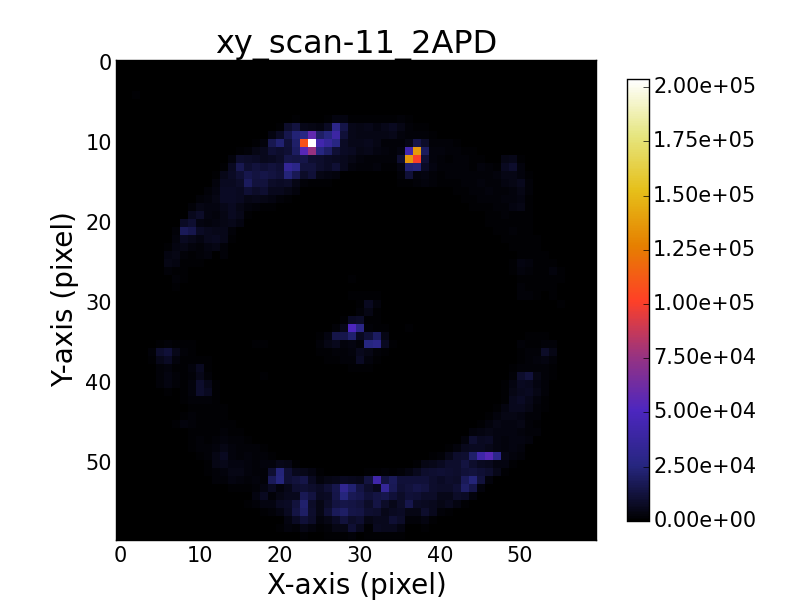
\includegraphics[trim = 0 0 0 0,  clip= true, width = \textwidth]{./pics/xy_scan-11_2APD.png}}
					\caption{}
					\label{subfig::antenna_laser_scan}
				\end{subfigure}
				\hfill
				\begin{subfigure}[t]{ 0.49\linewidth}
					\centering
					\testbox{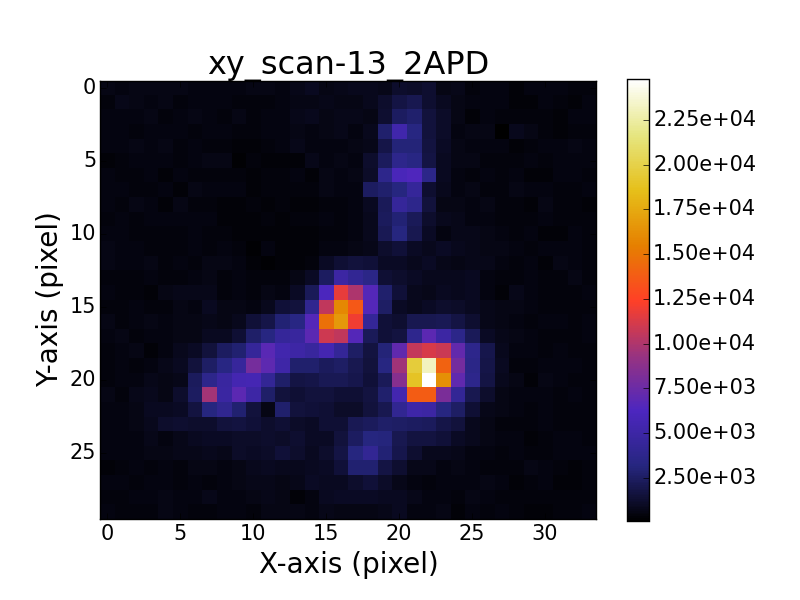
\includegraphics[trim = 0 0 0 0,  clip= true, width = \textwidth]{./pics/xy_scan-13_2APD.png}}
					\caption{}
					\label{subfig::antenna_bowtie_laser_scan}
				\end{subfigure}
				\caption[Confocal scan of a gold double bowtie antenna]{(a) Confocal scan of the double bowtie antenna where a \nd containing multiple \sivs had been placed. The rings are visible. (b) Detail scan of the triangles of the same antenna structure, which make up the double bowtie antenna. While the seperate triangle cannot be seen, some edges and two bright spots are visible. To identify the place of the \nd we compare the middle point of the rings in (a), the point of intersection of the edges and the bright spot and conclude that the upper bright spot in (b) is the location of the \nd. }
			\end{figure}

			These images suffices to approach the \nd close enough to measure a PL spectrum.
			The PL spectrum of the \siv in the nanodiamond gives insight to the effect of the nanoantenna on its emission.
			The result is displayed in \autoref{subfig::spectrum_antenna_nd_multiple}.

			To rule out artifacts, a spectrum of an antenna of the same dimensions without \nd is recorded (\autoref{fig::spectrum_antenna_no_nd}).
			% Fig. 7a where an increase in the PL intensity is observed by more than a factor 10 indicating that the nanoantennas indeed contribute to the enhancement of the SiV centers emission.
			% A $\lambda$ = 710 nm long pass filter is used to eliminate any signal from the laser.
			The additional peak at a lower wavelength is attributed to the antenna resonance mode.

			\begin{figure}[tp]
				\centering
				\testbox{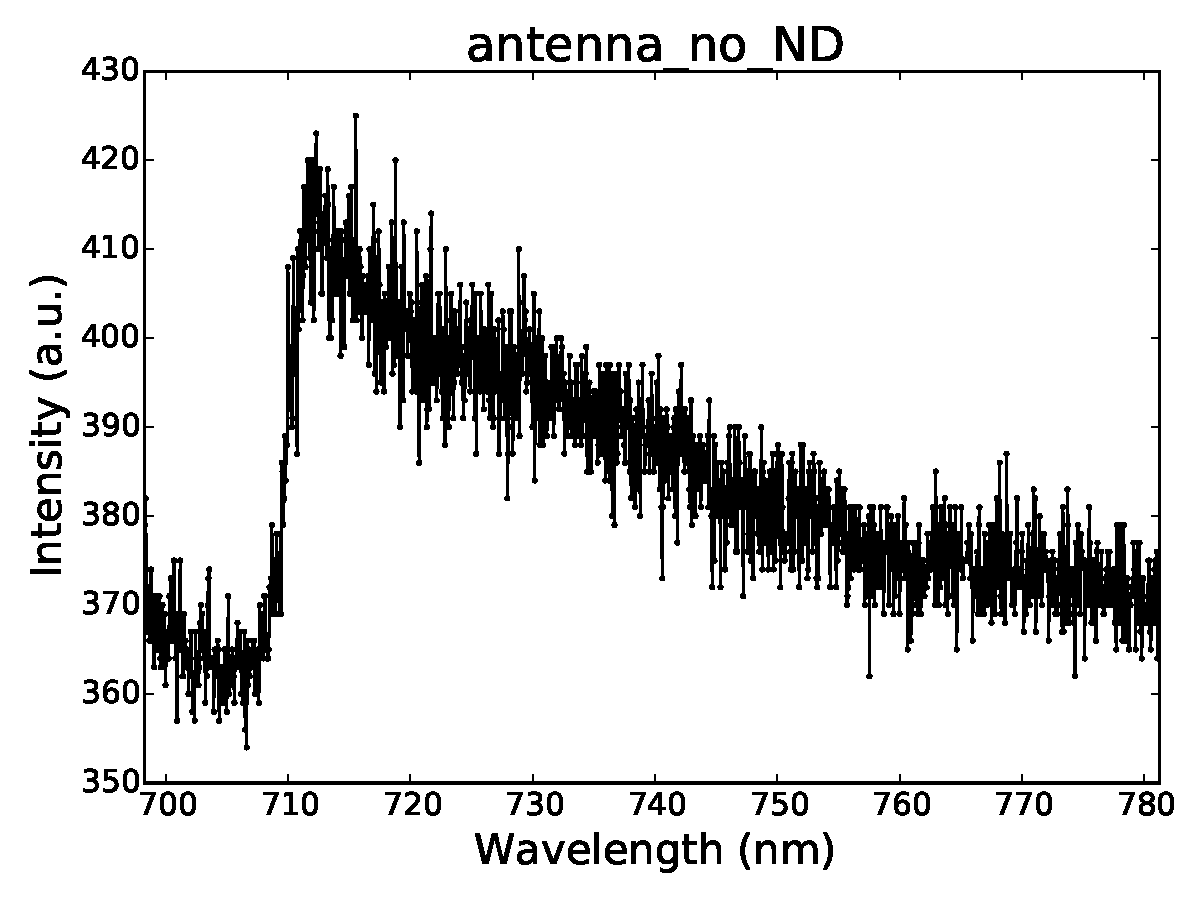
\includegraphics[trim = 0 0 0 0,  clip= true, width = 0.3\textwidth]{./pics/antenna_no_ND.pdf}}
				\caption{}
				\label{fig::spectrum_antenna_no_nd}
			\end{figure}


			To verify this, we convolute the experimental PL spectrum of the nanodiamond measured before placing it in the nanoantenna (\autoref{fig::spectrum_nd_multiple}) with the intensity spectrum of the nanoantenna obtained by simulations (\autoref{fig::antenna_fdtd_calculation}).
			The resulting spectrum is given in \autoref{subfig::antenna_convolution}, and is in good agreement with the measured spectrum in \autoref{subfig::spectrum_antenna_nd_multiple}, confirming that indeed the extra peak is due to the antenna resonance.

			\begin{figure}[htp]
				\begin{subfigure}[t]{ 0.49\linewidth}
					\centering
					\testbox{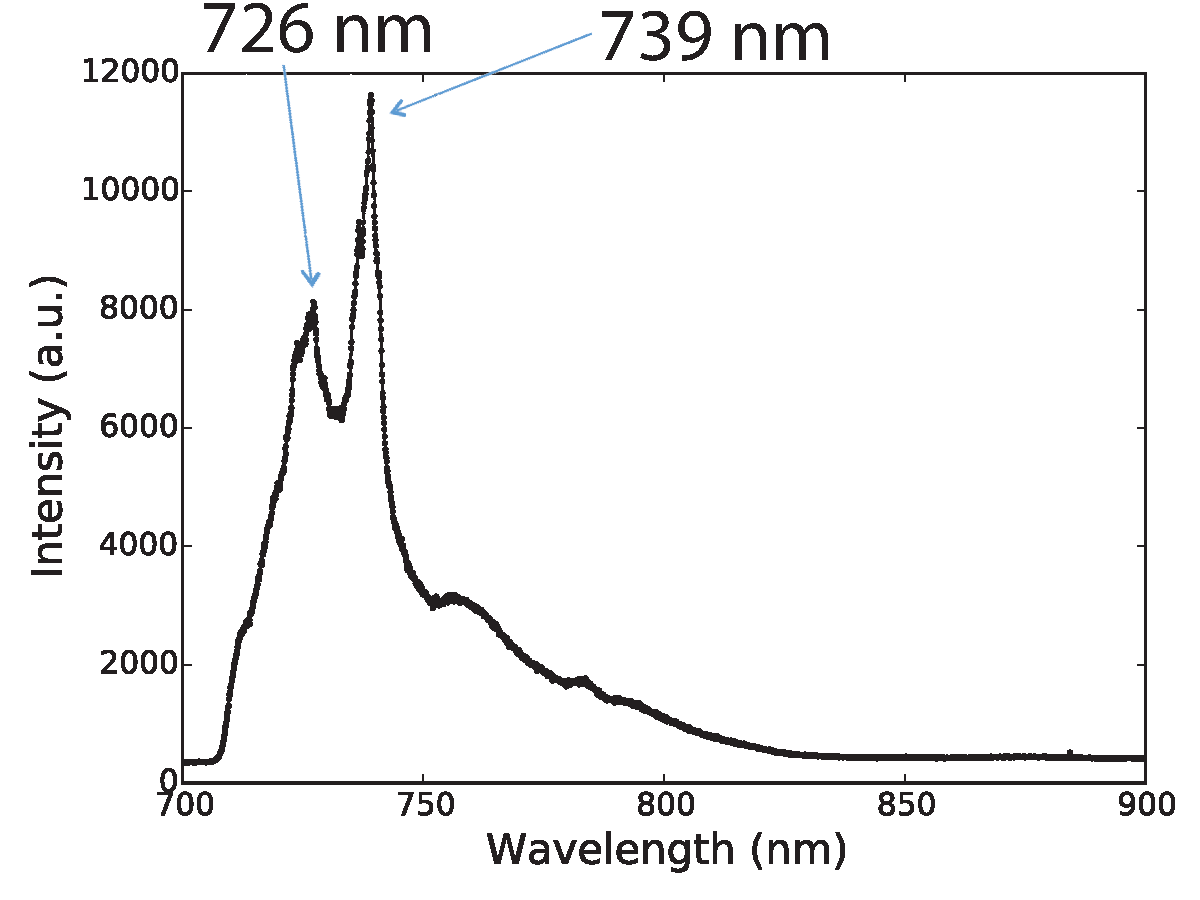
\includegraphics[trim = 0 0 0 0,  clip= true, width = \textwidth]{./pics/find_middle_with_ccd_highP_2_arrows.pdf}}
					\caption{}
					\label{subfig::spectrum_antenna_nd_multiple}
				\end{subfigure}
				\hfill
				\begin{subfigure}[t]{ 0.49\linewidth}
					\centering
					\testbox{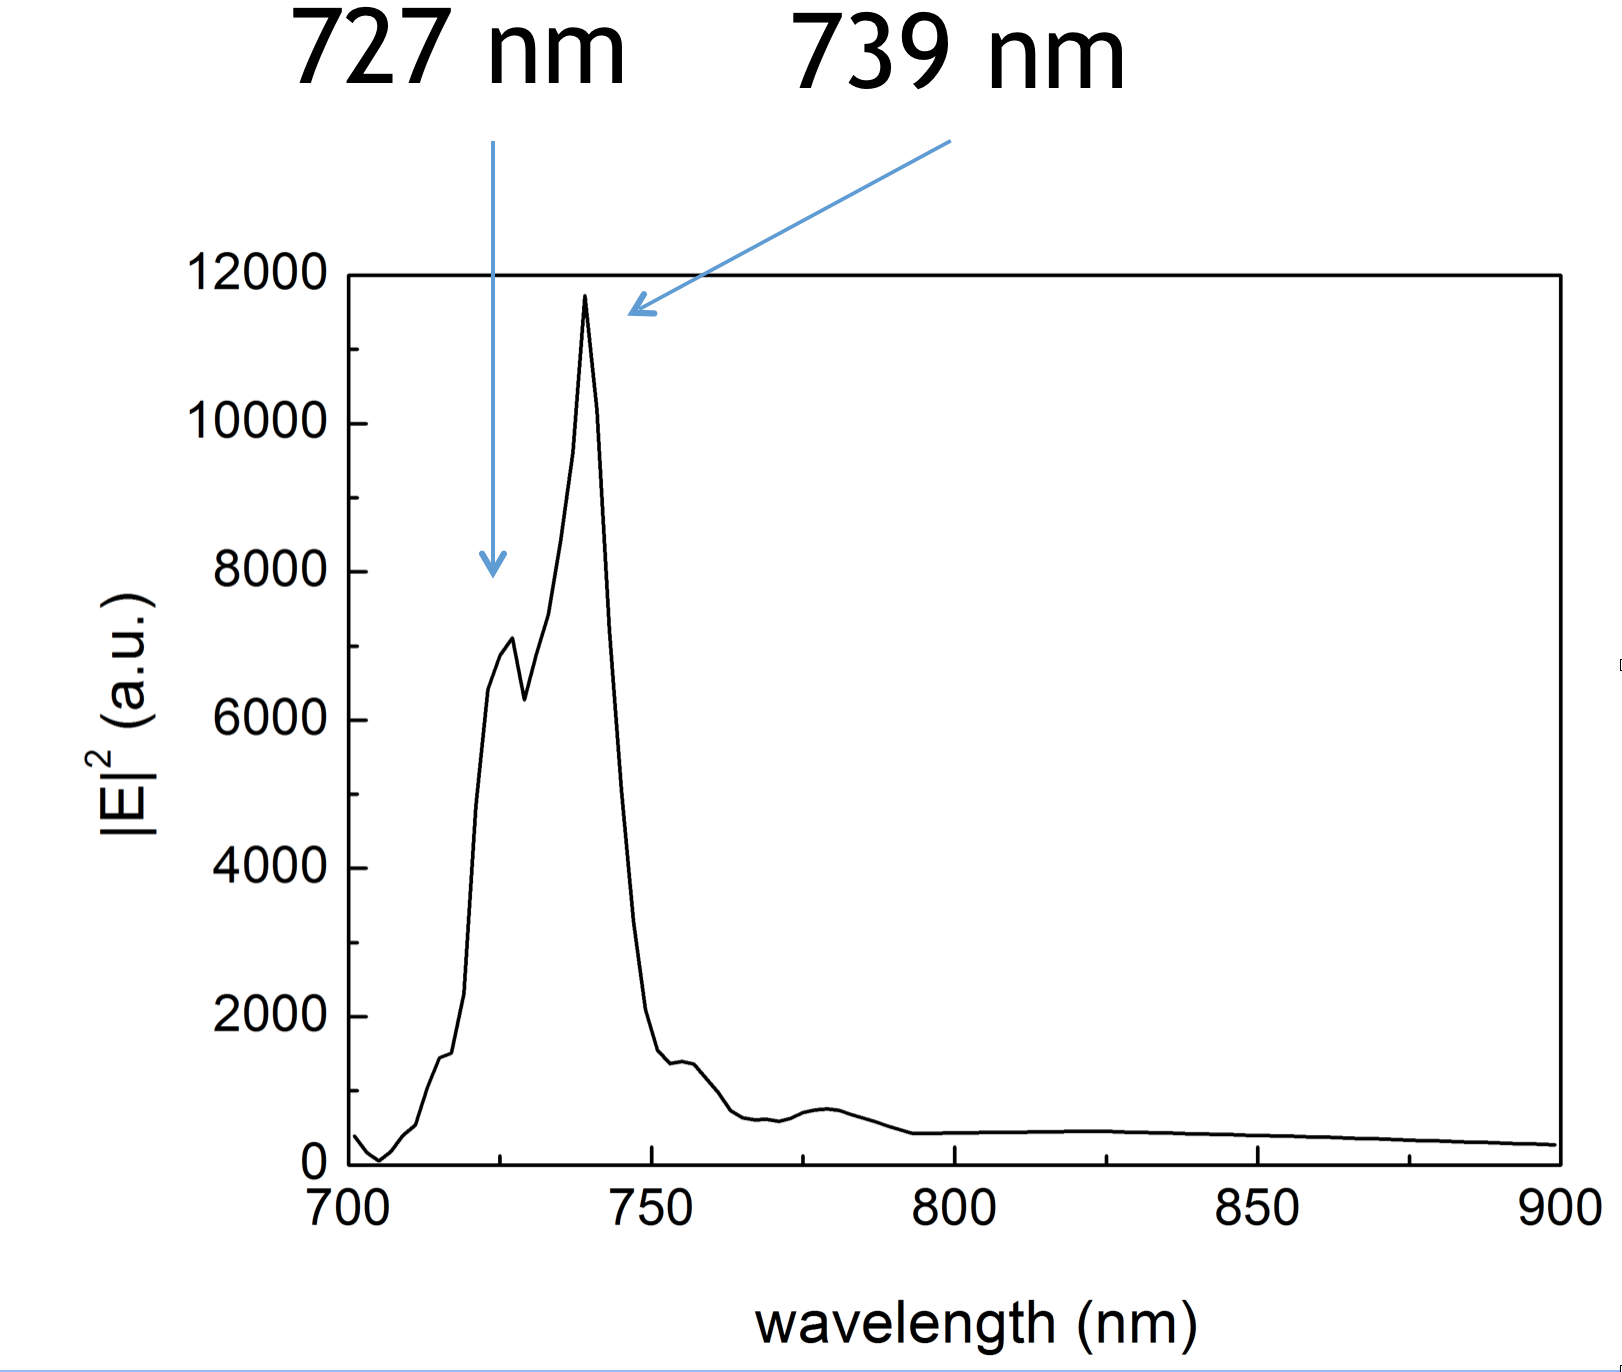
\includegraphics[trim = 0 0 0 0,  clip= true, width = \textwidth]{./pics/antenna_convolution.png}}
					\caption{}
					\label{subfig::antenna_convolution}
				\end{subfigure}
				\caption{(a) Measured PL spectrum of the emitter after placing the \nd into the nanoantenna, (b) Convolution of the spectrum of the measured PL spectrum of the emitter before \pp (see \autoref{fig::spectrum_nd_multiple}) and the simulated resonance spectrum of the nanoantenna (see Figure \autoref{fig::antenna_fdtd_calculation}).}
			\end{figure}

			Kopplung experimentell machbar.
			Kopplung erfolgreich - simulation in agreement with measuerments.
			Enhancement nicht quantifizierbar weil ensemble of emitters.



		\subsubsection{\Nd With Few \siv Coupled to Antenna}\label{subsubsection::antenna_single_siv}

			As the experiment of coupling a \nd with an ensemble of \sivs proved to be very successful, the next step was to select a \nd with only few \sivs, i.e. that it exhibits countrate saturation and a dip in the \gtf.
			In this section, coupling a \nd containing only few \sivs to a double bowtie antenna is reported.
			It is an intermediate step between coupling
			% sample description
			The origin sample used for this experiment is an \ir substrate onto which a solution of \nds were drop-casted.
			Starting material for the \nds was a electronic grade diamond film produced by the company rho-BeSt coating (now CarbonCompetence)\todo{checken, ob angaben passen}.
			It was then milled in a \basd process\footnote{\krueger} to \nds of a size of \todo{groesse einfuegen}.
			The \nds were drop-casted at \SI{60}{\celsius} onto an \ir substrate containing cross markers which had been treated with Piranha etch.
			% sample M02-16: drop-casted with SiGH45
			\\
			% preselection,
			Preselecting a \nd with a single \siv is imposes additional constrains to the suitability of an \nd if compared to a \nd with multiple \sivs.
			First, only a small percentage of the technically suited \nds (size, isolation) contain a single \siv, second, damage due to electon radiation during \pp.
			% position
			The position of the \sivs on the substrate surface was performed in the same way as described in \autoref{subsubsection::
			}.
			The identification whether bright spots in the scan were suitable emitter was performed as follows:
			First a saturation curve was recorded.
			Countrate saturation is only a necessary and not a sufficient measure for single photon emission, hence the saturation measurement alone does not prove that the emitter in question is single.
			However, it takes only a few seconds to record a saturation measurement compared to potentially hour-long measurements of \gtfs.
			Therefore, it is a quick selection method to evaluate potential candidates.
			Once an emitter with a saturating countrate was found, a spectrum was recorded to prove that the emitter in question is indeed an \siv.
			At last, the \gtf was recorded.
			We successfully found an \siv with a small dip in the \gt function.
			While the dip is too small to account for a single \siv, it indicates the presence of only few \sivs.
			% transfer
			Hence, we proceeded by transferring the host \nd to the antenna structure.
			\\
			% Spectroscopic measurements
			The \siv coupled to the antenna structure was then spectroscopically investigated in the confocal setup.
			First, we recorded a spectrum (spectrum A).
			The result of the first recorded spectrum revealed a multitude of peaks.
			To ensure that the peaks are no artifacts due to deficient alignment, we rechecked the alignment which proved to be precise.
			We initiated another measurement of the spectrum.
			However, this time the recorded spectrum only showed a broad \bkg (spectrum B).
			After checking in the confocal scan that the measurement was performed at the correct position, we had to conclude that the emitter bleached shortly after recording spectrum A.
			\\
			As mentioned earlier, the electron radiation may damage \sivs in nanodiamonds.
			The electron radiation might have put the \siv into an unstable state.
			Although we were still able to measure one spectrum, further application of energy from the laser seems to have permanently bleached the \siv.
			While we cannot solidify this conclusion with further experimental evidence, we observed in earlier independent measurements that some \sivs bleach after electron radiation and that some \sivs bleach after an extended laser irradiation \cite{}.
			The observations in this measurement suggest a combination of the two effects.
			\\
			We performed FDTD calculations of the selected \siv in the host \nd in the plasmonic double bowtie antenna as described in the previous section\todo{put in pictures}.
			We used spectrum B to for \bkg correction of spectrum A and fitted the measured peaks (\autoref{subfig::single_siv_spec_after_transfer_antenna_bkg_corrected}).
			In the simulations, we do not see the peaks between \SIrange{700}{750}{nm} that we recorded in the measurement.
			Hence, we conclude, that not additionally to the observed photobleaching, also the emitter's spectrum was modified in the \pp process.
			While it is not possible to pinpoint exactly which circumstance caused the modification, possible candidates are\todo{enter candidates and explain why}.
			\\
			To gain further insight, we performed FDTD calculations with antenna damage and different dipole orientation.
			To be able to include the dipole orientation into the calculations, a dipole emitter with a broad emission instead of a narrow emission peak has to be used.
			Therefore, the convolution method as described in the previsous section is more adequate for our purpose, as the \siv exhibits a very narrow emission peak.
			However, these calculations give further insight.
			First, the antenna damage does not have a big effect on the spectra, however the dipole orientation changes the results drastically (\autoref{}).
			Therefore, future experiments should include polarization measurements to experimentally quantify the impact of the emitter orientation.

			\begin{figure}[tp]
				\begin{subfigure}[t]{ 0.49\linewidth}
					\centering
					\testbox{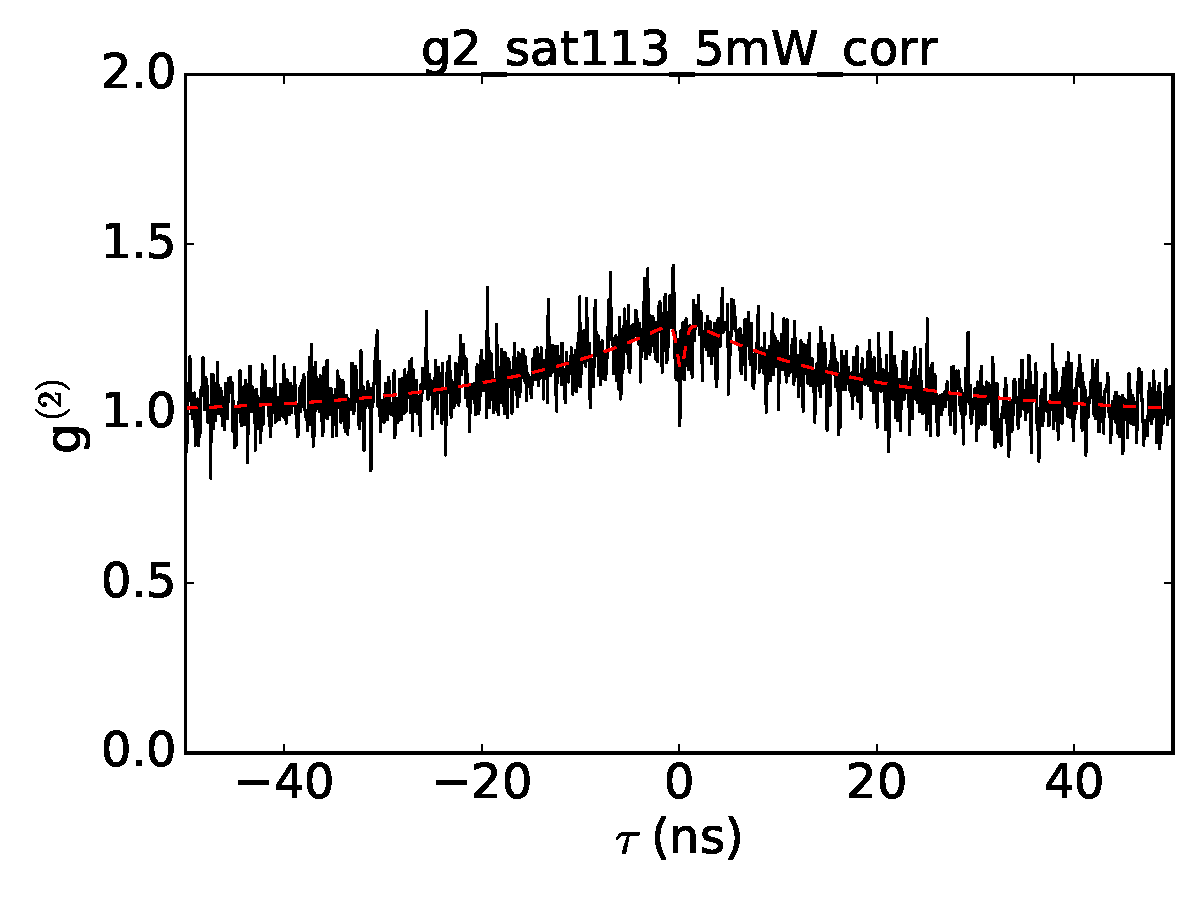
\includegraphics[trim = 0 0 0 0,  clip= true, width = \textwidth]{./pics/g2_sat113_5mW_corr_fit.pdf}}
					\caption{}
					\label{subfig::single_siv_g2_before_transfer_antenna}
				\end{subfigure}
				\hfill
				\begin{subfigure}[t]{ 0.49\linewidth}
					\centering
					\testbox{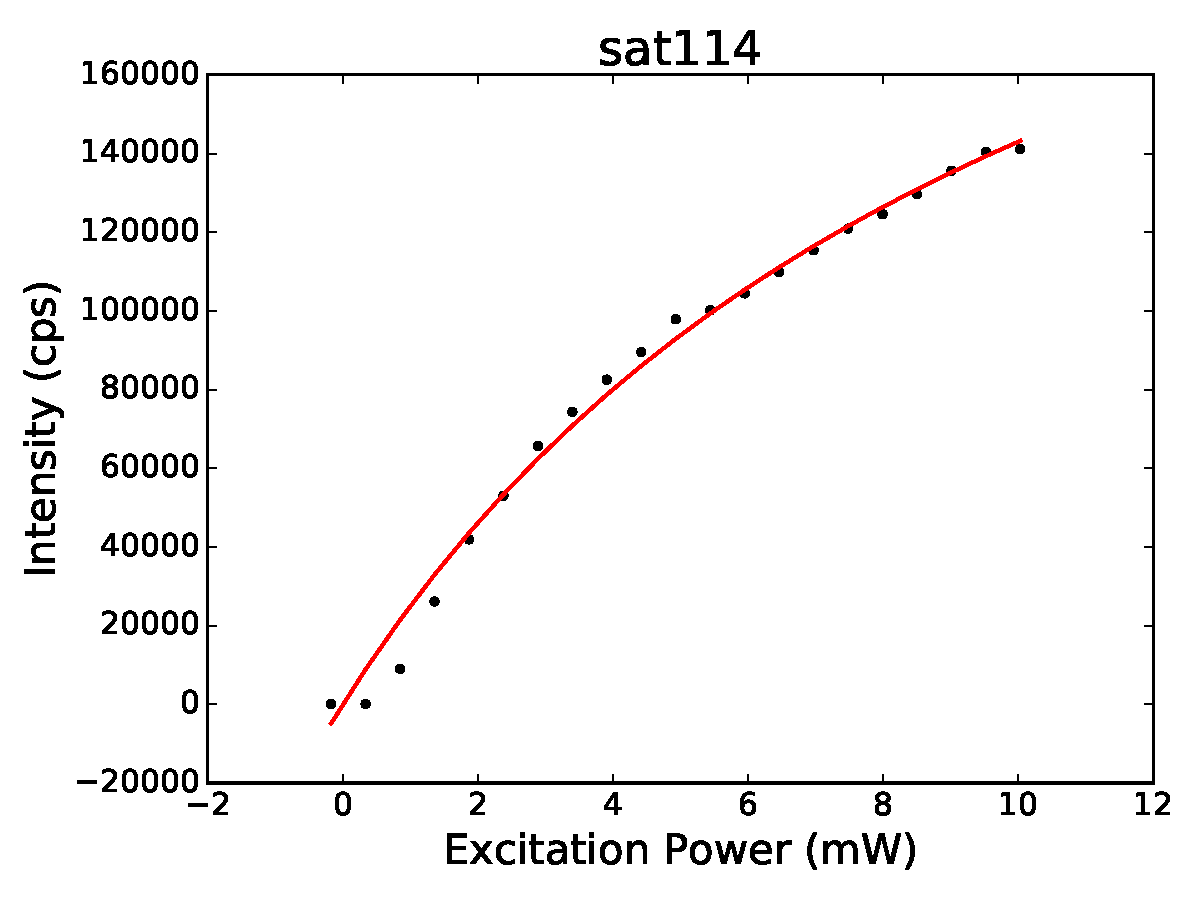
\includegraphics[trim = 0 0 0 0,  clip= true, width = \textwidth]{./pics/sat114_fit_bkg.pdf}}
					\caption{}
					\label{subfig::single_siv_sat_before_transfer_antenna}
				\end{subfigure}
				\caption{(a) The \gtf of the preselected \nd hosting few nanodiamonds. A dip at \gtz is present, however it does not decrease below 0.5. While this indicates that more than one \siv is present, a small number of \sivs cause a dip in the \gtf instead of no dip at all which would be measured under coherent emission\todo[inline]{cps zu a.u. aendern}. (b) Saturation curve of the same emitter\todo[inline]{zahlen fuer sat eintragen}. Data points are black, fitted curve red.}
			\end{figure}

			\begin{figure}[tp]
				\begin{subfigure}[t]{ 0.49\linewidth}
					\centering
					\testbox{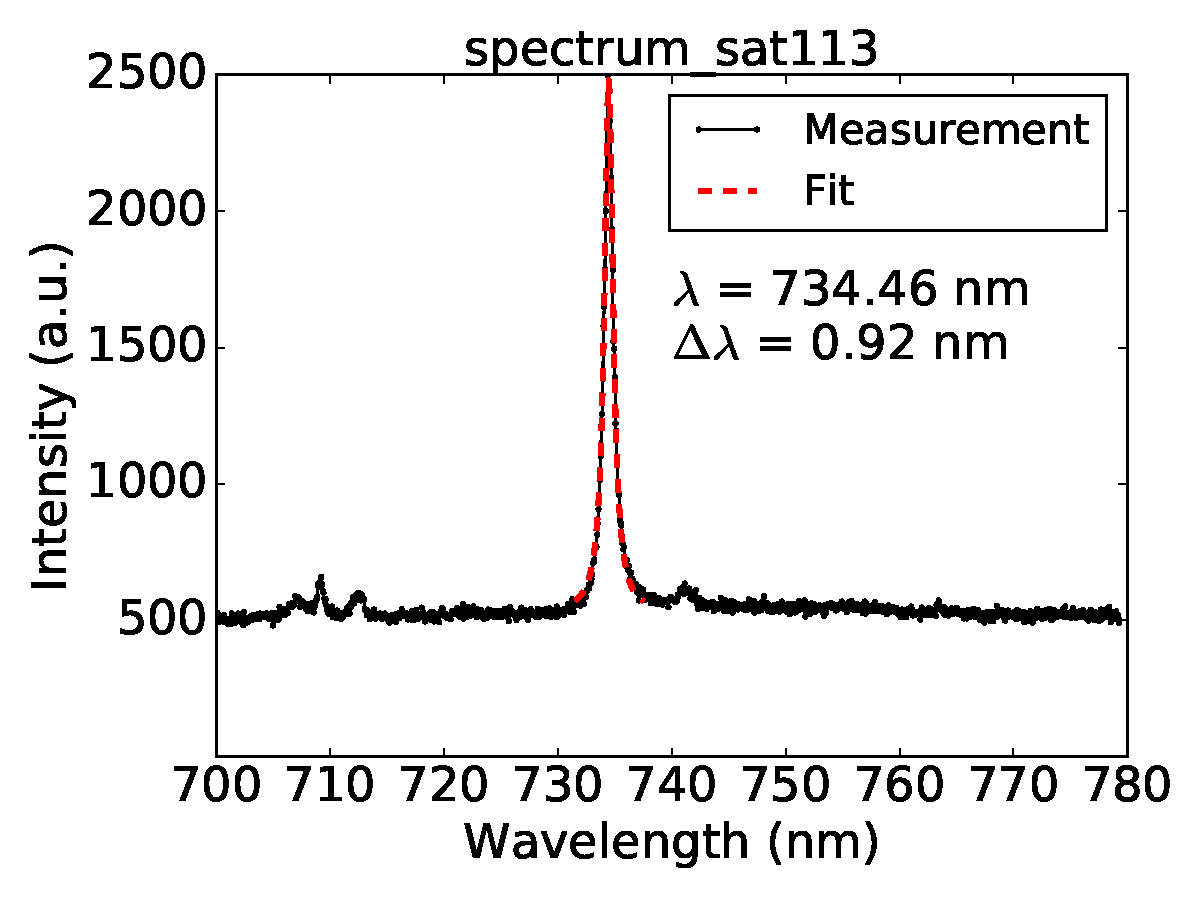
\includegraphics[trim = 0 0 0 0,  clip= true, width = \textwidth]{./pics/single_spectrum_sat113_fit.pdf}}
					\caption{}
					\label{subfig::single_siv_spec_before_transfer_antenna}
				\end{subfigure}
				\hfill
				\begin{subfigure}[t]{ 0.49\linewidth}
					\centering
					\testbox{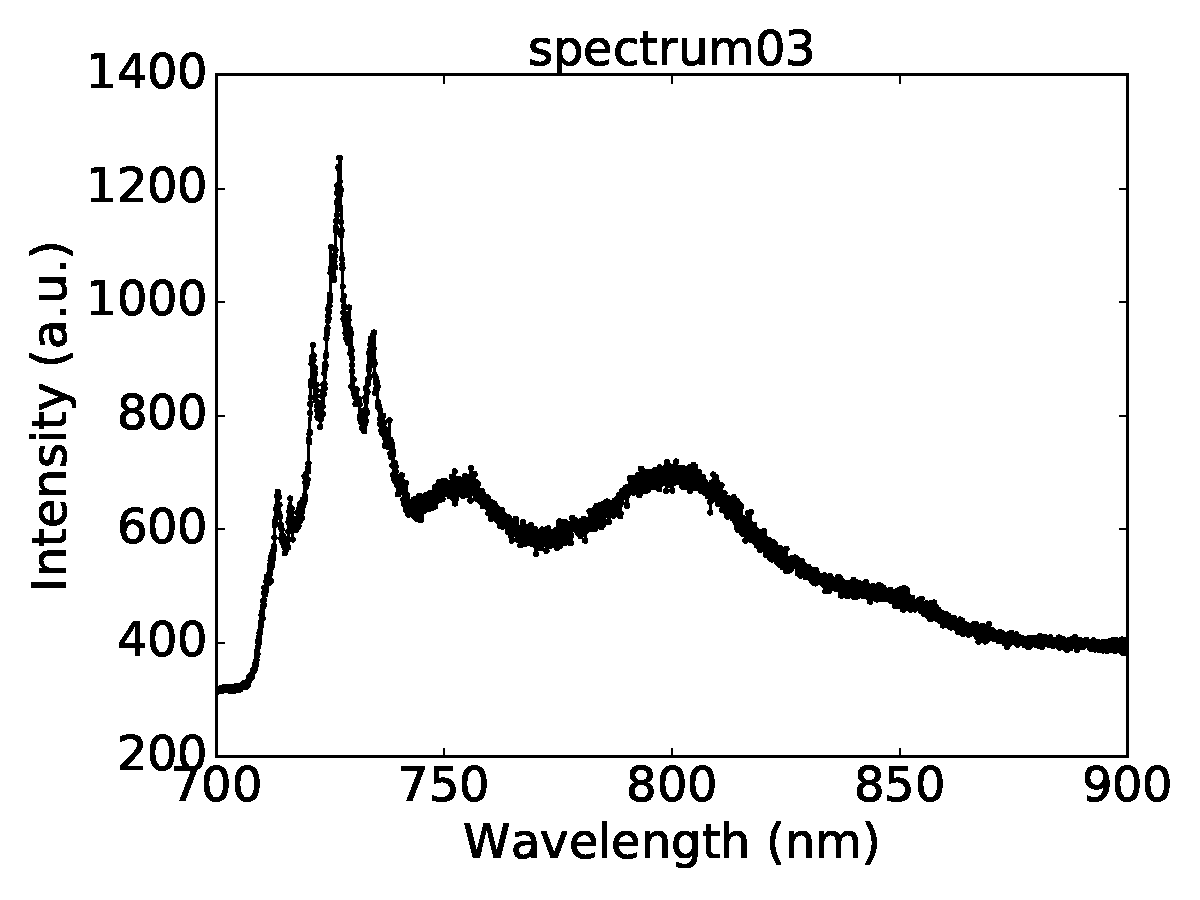
\includegraphics[trim = 0 0 0 0,  clip= true, width = \textwidth]{./pics/spectrum03.pdf}}
					\caption{}
					\label{subfig::single_siv_spec_after_transfer_antenna}
				\end{subfigure}
				\caption{(a) Spectrum of the preselected \nd hosting few \sivs. (b) Measured spectrum after transfer of the preselected \nd into the double bowtie antenna.}
			\end{figure}

			% \begin{figure}[tp]
			% 	\centering
			% 	\testbox{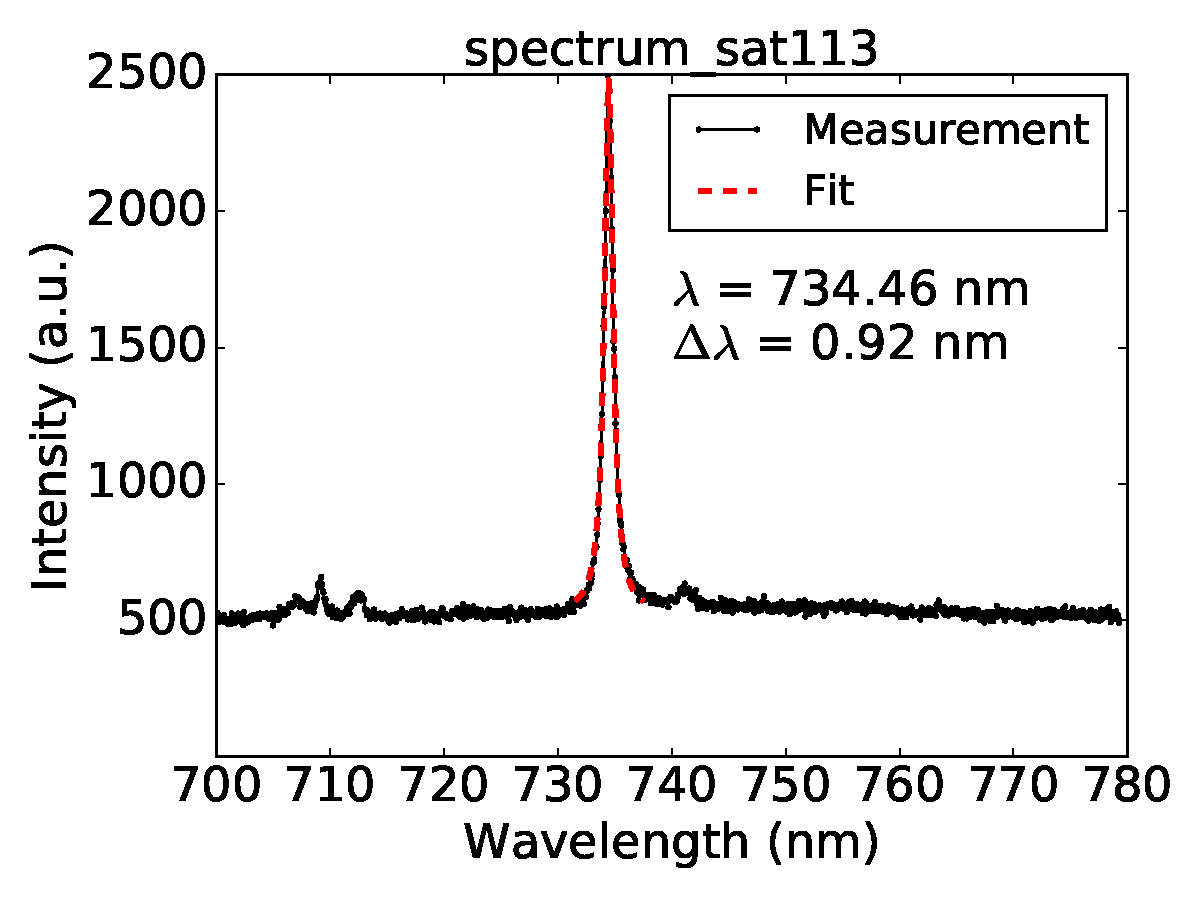
\includegraphics[trim = 0 0 0 0,  clip= true, width = 0.5\textwidth]{./pics/single_spectrum_sat113_fit.pdf}}
			% 	\caption{<caption>}
			% 	\label{fig::single_siv_spec_before_transfer_antenna}
			% \end{figure}

			\begin{figure}[tp]
				\begin{subfigure}[t]{ 0.49\linewidth}
					\centering
					\testbox{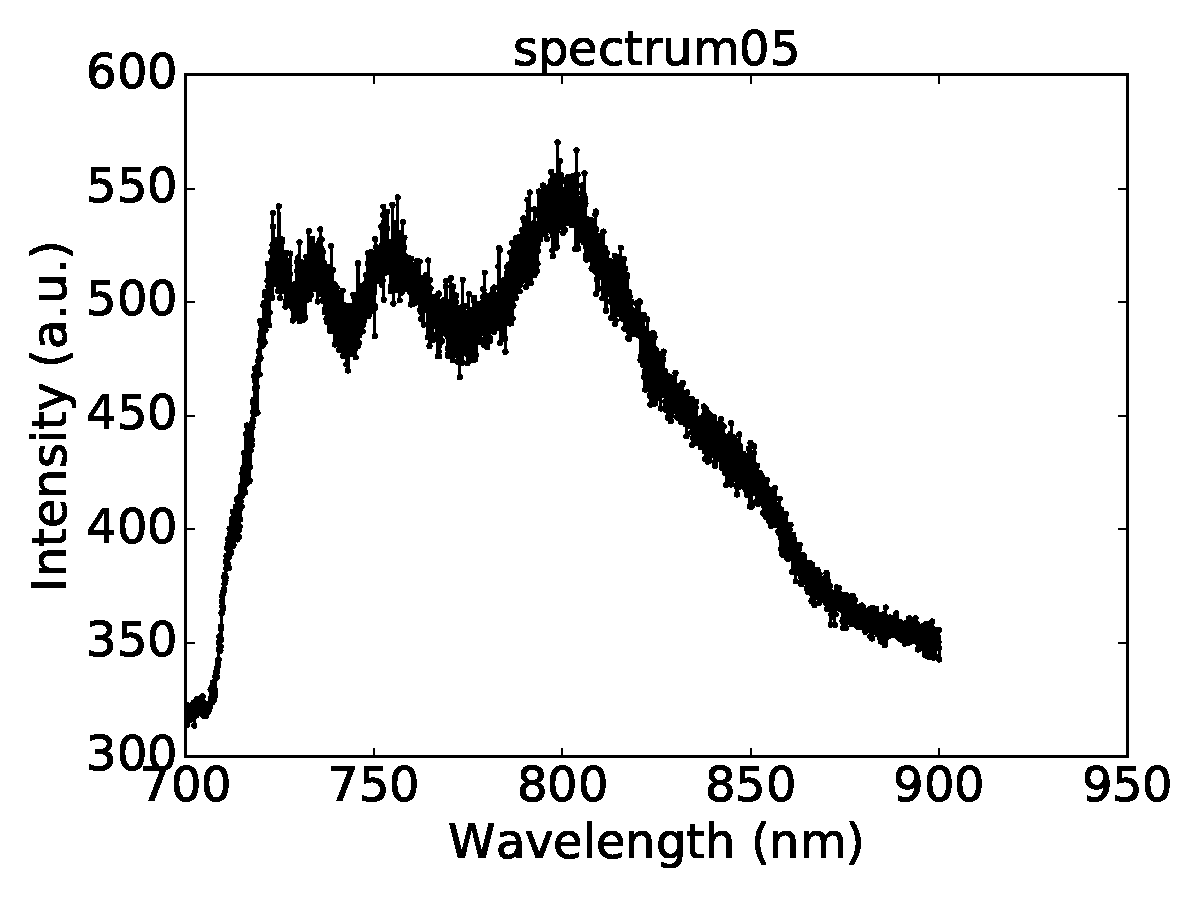
\includegraphics[trim = 0 0 0 0,  clip= true, width = \textwidth]{./pics/spectrum05.pdf}}
					\caption{}
					\label{subfig::single_siv_spec_bkg_antenna}
				\end{subfigure}
				\hfill
				\begin{subfigure}[t]{ 0.49\linewidth}
					\centering
					\testbox{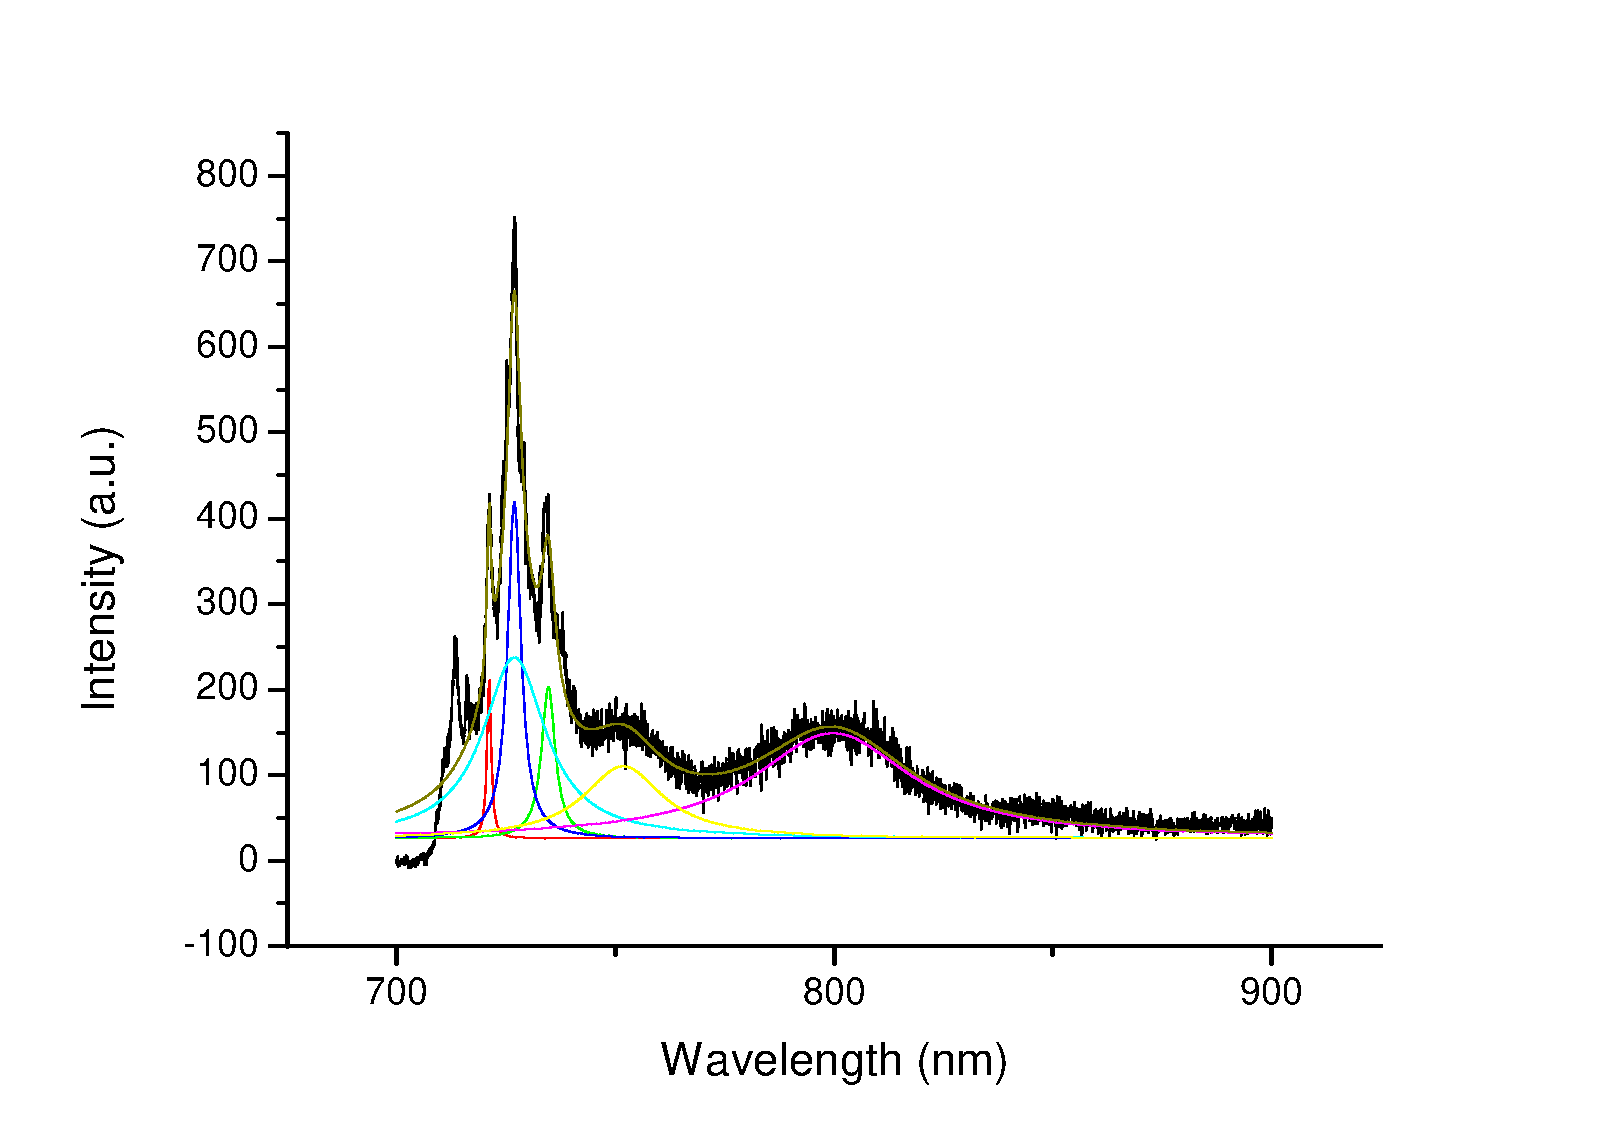
\includegraphics[trim = 0 0 0 0,  clip= true, width = \textwidth]{./pics/spectrum_sat113_fit_origin.pdf}}
					\caption{}
					\label{subfig::single_siv_spec_after_transfer_antenna_bkg_corrected}
				\end{subfigure}
				\caption{(a) Spectrum of the \nd hosting few \sivs coupled to the double bowtie antenna after the emitter bleached. (b) Background corrected spectrum of the transferred \nd in the double bowtie antenna. Peaks are fitted, results of the fits are the colored lines. For background correction, the spectrum in (a) was used.}
			\end{figure}

		\subsubsection{Outlook: Coupling a \Nd With a Single \Siv to the Plasmonic Double Bowtie Antenna}
			To effectivly state the emission enhancement of the \siv by the plasmonic double bowtie antenna, a single \siv is necessary.
			A correct measure for the emission enhancement is the saturation count rate.
			The saturation countrate is proportional to the inverse of the emitter's lifetime.
			Hence, if there are two or more emitters present, photons of the individual emitters are emitted randomly, which renders a correct saturation measurement impossible.
			However, finding \sivs in \nds which fulfill both spectroscopic (\gtz $\approx$0, saturation, narrow \ZPL spectrum) and technical (size, isolation of \nds) constraints tured out to be a very time-consuming work.
			\\
			We investigated different kinds of \nds in the search of \nds exhibiting optimal spectroscopic and technical parameters.
			We were able to fulfill the size requirements posed by the \pp process and antenna design by producing different patches of different sizes of \nds and took the ones which were best suited.
			We also developped a good isolation of the \nds on the substrate by treating the \ir substrate with Piranha etch and tuning the amount of diamond solution drop-casted onto the substrate.
			This leaves us with the need of a higher propability of exactly one \siv per \nd.
			Parameters which have an impact on the quantity of \sivs per \nd are the initial \siv density in the starting material and the \nd size.
			Once the time constraint of finding a single \siv in a \nd is overcome, we can apply the extensive methods and knowledge gained by the reported procedures to couple a single \siv to a plasmonic bowtie antenna.
			\\
			To our knowledge, our experiments were the first time an \siv in a \nd was coupled to a plasmonic bowtie antenna.
			The extraordinarily precise correlation of the theoretically predicted and the experimentally recorded spectrum of an ensemble of \sivs in a \nd make this process a promising candidate for future applications.
